\section{Methods}
 Two different methods were used in this assignment, Correlation detection and Goertzel -algorithm. In the first method we calculated the correlation between the input data and and the signals ~\ref{eq:cos} and ~\ref{eq:sin}.

\begin{equation}
  \label{eq:cos}
  c_{697}(n) = \cos(2 \pi \times 697 \times n/F_{n})
\end{equation}

\begin{equation}
  \label{eq:sin}
  s_{697}(n) = \sin(2 \pi \times 697 \times n/F_{n})
\end{equation}

The correlations are defined by equations ~\ref{eq:corCos} and ~\ref{eq:corSin}.

\begin{equation}
  \label{eq:corCos}
  c_{\cos}(697) =\sum_{n=0}^{N-1} c_{697}(n)  \times x(n)
\end{equation}

\begin{equation}
  \label{eq:corSin}
  c_{\sin}(697) =\sum_{n=0}^{N-1} s_{697}(n)  \times x(n)
\end{equation}

Next we estimated the signal power using equation ~\ref{eq:var}.

\begin{equation}
  \label{eq:var}
  var =\sum_{n=0}^{N-1}x(n)^2
\end{equation}

Finally, we tested the presence of the frequency using equation ~\ref{eq:pres} In this case, we tested the presence of the 697Hz component. By replacing the 697 value in the equations, we can test the presence of the other components.

\begin{equation}
  \label{eq:pres}
 w_{697} =\frac {c^2_{cos}(697) + c^2_{sin}(697)}{var}
\end{equation}

The resulting LabVIEW can be seen in figure ~\ref{fig:correlation}

\begin{figure}[H]
  \centering
  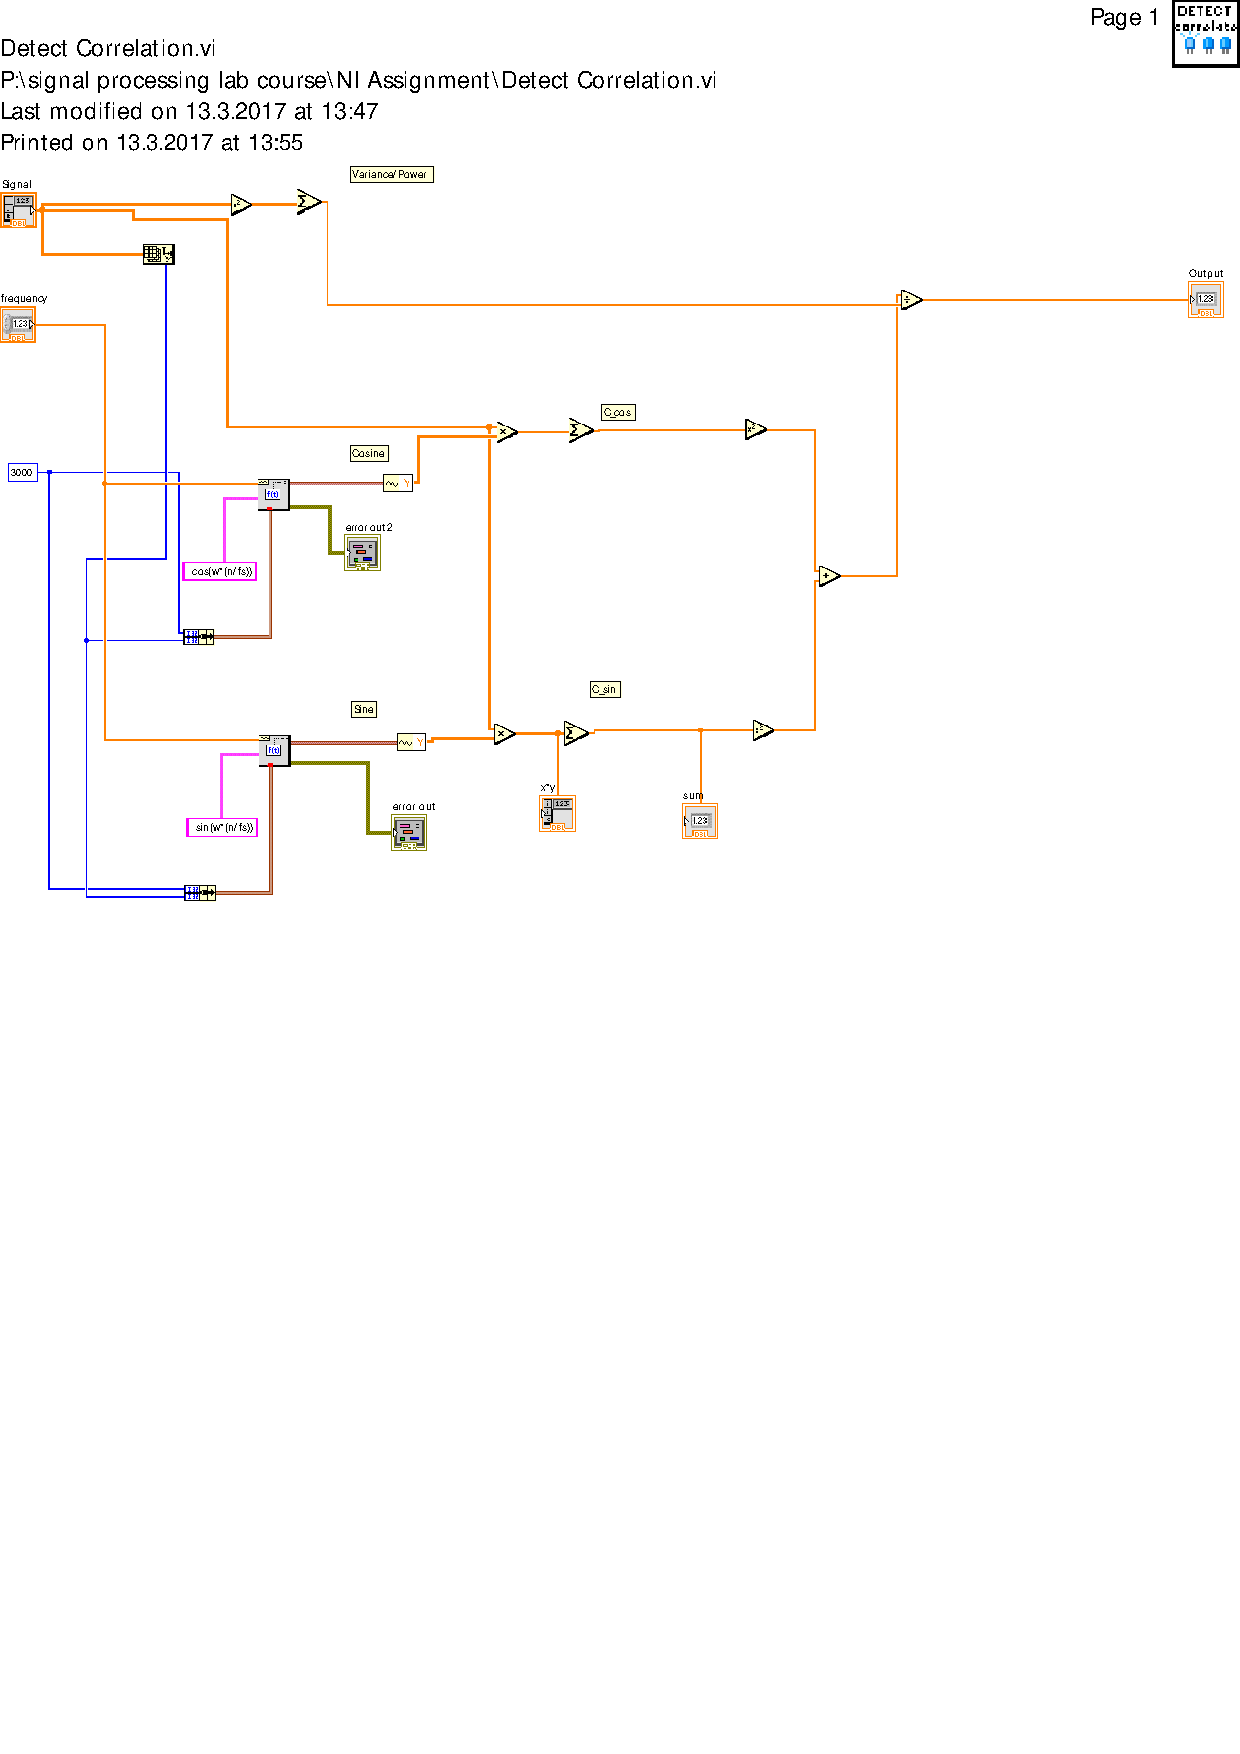
\includegraphics[width=0.8\linewidth]{detect_freq}
  \caption{LabVIEW code for Detect Correlation}
\label{fig:correlation}
\end{figure}


The Goertzel-algorithm uses an unstable IIR filter that amplifies the selected frequencies. Detecting the frequency f with sampling frequency $F_{s}$ can be done using Goetzel filter ~\ref{eq:gFilter}.

\begin{equation}
  \label{eq:gFilter}
  y(n) =x(n) + 2\cos(2 \pi f/F_{s})y(n-1) - y(n-2)
\end{equation}

\begin{equation}
  \label{eq:gFilter}
  y(n) =x(n) + 2\cos(2 \pi f/F_{s})y(n-1) - y(n-2)
\end{equation}

However, we cannot use this equation as a direct indication on which LED should light. Instead, we can use equation ~\ref{eq:gFinal}.

\begin{equation}
  \label{eq:gFinal}
  |Y(e^{(i \omega)}|^2 = y^2(N-1) + y^2(N-1) - 2 \cos(2 \pi f/F_{s})y(N-2)y(N-1)
\end{equation}

The Goertzel algorithm itself consists of three steps. We loop through all the steps, increasing the value of n with every step. Step 1. we initialize n , y(n-1) and y(n-2) as 0. Then in step 2, if n < N we calculate y(n) using ~\ref{eq:gFilter}, increment n = n+1 and return to step 2.In step 3, if n  is equal to N,  we calculate ~\ref{eq:gFinal}. and divide it with variance, using equation ~\ref{eq:var}.
This value is compared to the thresholdn and if it is greater than the threshold, LED is turned on, otherwise it's turned off. Again, we increment n=n+1 and return to step 1


\begin{figure}[H]
  \centering
  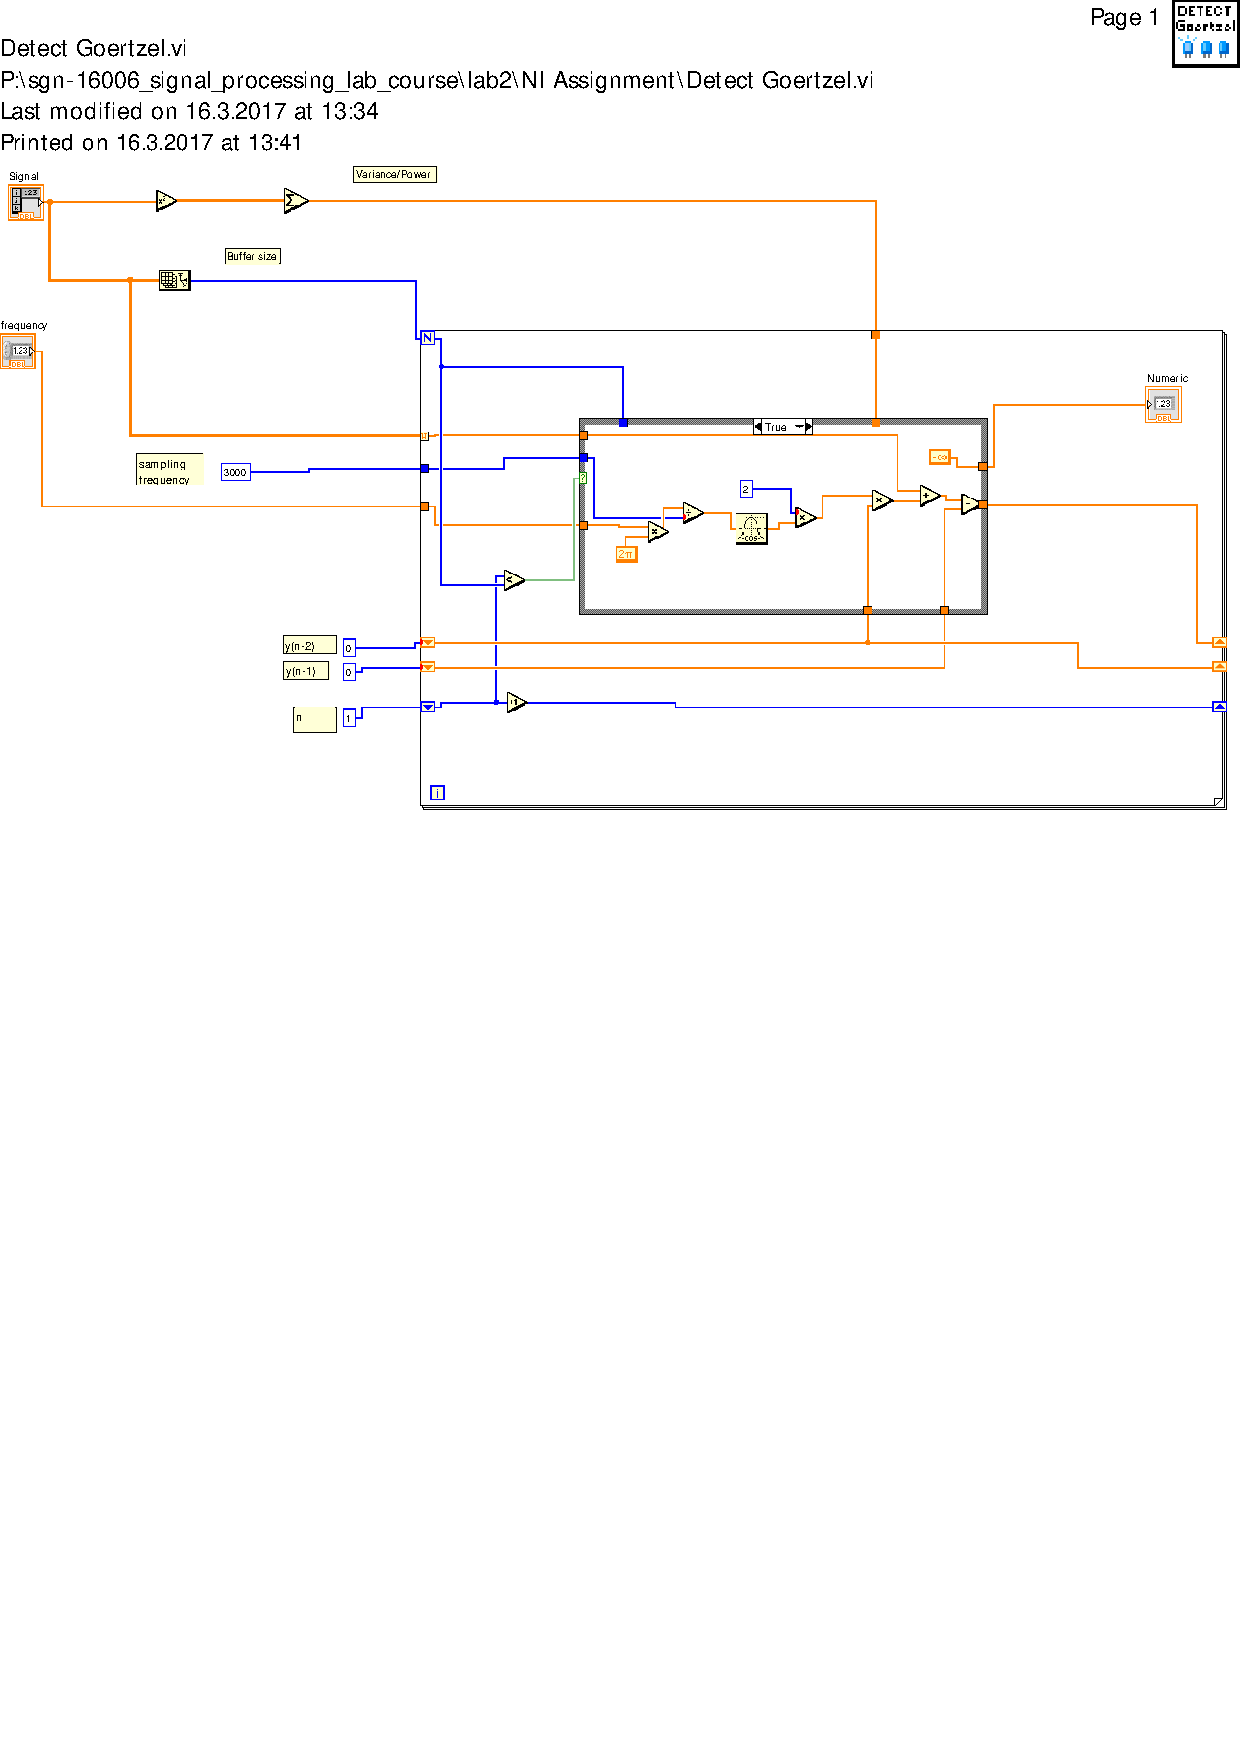
\includegraphics[width=0.8\linewidth]{detect_goertzel_true}
  \caption{Goertzel-algortihm in LabView when n $<$ N}
\label{fig:GoertzelTrue}
\end{figure}


\begin{figure}[H]
  \centering
  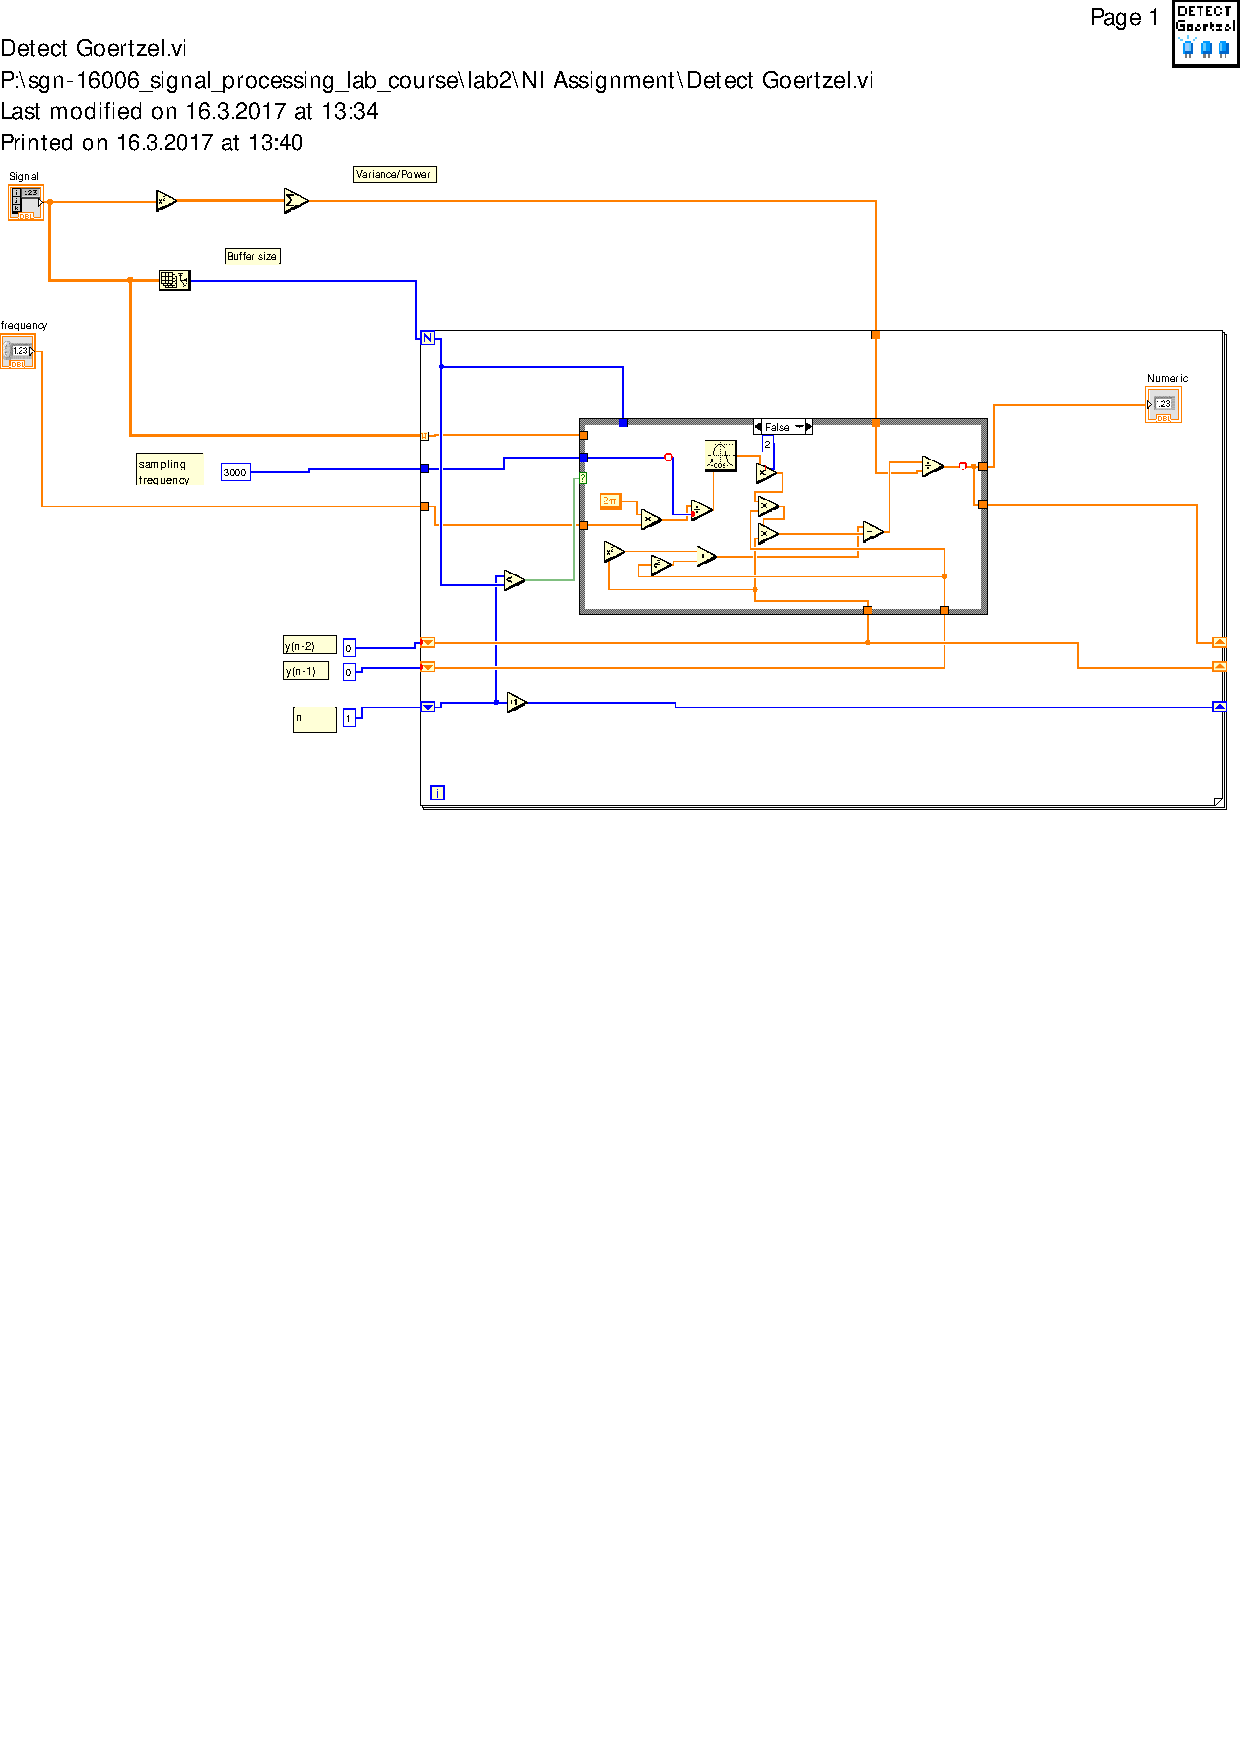
\includegraphics[width=0.8\linewidth]{detect_goertzel_false}
  \caption{Goertzel-algortihm in LabView when n = N}
\label{fig:GoertzelFalse}
\end{figure}

